\section{Funktionaler Vergleich der Spracherweiterungen}
\label{vergleich}

\subsection{Anforderungen an Spracherweiterungen}
\label{vergleich:anforderungen}

Ein Vergleich der Fähigkeiten der einzelnen Spracherweiterungen erfordert einen
Kriterienkatalog, anhand dessen die Bewertung erfolgen kann. Dabei sind sowohl
die Sicht auf die Daten, also der Umgang der Spracherweiterungen mit den Daten,
als auch die Sicht auf die Aufgaben, also die Transformation der Daten, zu
berücksichtigen.

\subsubsection{Datensicht}
\label{vergleich:anforderungen:datensicht}

Der effiziente Umgang mit großen Datenmengen ist seit jeher eines der
Kernprobleme des \gls{hpc} im Allgemeinen und heterogener Systeme im Besonderen,
d.h.\ unterschiedlicher Berechnungs-Hardware im selben Rechnersystem. Michael
Wong\footnote{Mitglied des C++-Standard-Komitees, ehemaliger Projektleiter des
XL-C++-Compilers der Firma IBM und derzeit Entwicklungsleiter des Unternehmens
Codeplay, das unter anderem den SYCL-Standard implementiert} bezeichnete in
einem Vortrag im November 2018 vor LLVM-Entwicklern die folgenden Punkte als
essentielle Probleme der Programmierung heterogener Systeme
(vgl.~\cite{wong2018}):

\paragraph{Datenbewegung} 
Die Bewegung der Daten ist stets mit Kosten verbunden. Im Allgemeinen ist damit
der Zeitbedarf gemeint, um Daten etwa vom Hauptspeicher des Systems in den
Speicher der GPU zu kopieren. Im weiteren Sinne kann dieser Punkt aber auch
andere Kriterien umfassen, wie z.B.\ den für den Kopiervorgang notwendigen
Energiebedarf, der als Bestandteil des gesamten Energiebedarfs von
\gls{hpc}-Systemen in jüngerer Zeit ebenfalls Gegenstand der Forschung geworden
ist.

Aus der Sicht des Programmierers ist außerdem die Frage relevant, ob die
Datenbewegung \textit{explizit} oder \textit{implizit} erfolgt. Die
\textit{explizite} Datenbewegung hat den Vorteil, dass der Programmierer
jederzeit die volle Kontrolle über die Verschiebung und damit auch über die
Performanz hat, geht jedoch mit einer höheren Programmierkomplexität und damit
Fehleranfälligkeit einher. Überdies wird die volle Kontrolle nicht
notwendigerweise an jeder Stelle gebraucht und bläht damit den Quelltext unnötig
auf. Die Adressräume bleiben bei der expliziten Datenbewegung getrennt (siehe
Abbildung~\ref{vergleich:anforderungen:datensicht:explizitebewegung})

Diesem Ansatz steht die \textit{implizite} Datenbewegung gegenüber. Diese
überlässt den Zeitpunkt und den konkreten Vorgang des Kopierens oder
Verschiebens sowie den Umfang der bewegten Datenmenge der Laufzeitumgebung; aus
Sicht des Programmierers existiert ein virtueller Adressraum, den sich CPU und
GPU teilen (siehe
Abbildung~\ref{vergleich:anforderungen:datensicht:implizitebewegung}).

\begin{figure}[!hbt]
    \centering
    \begin{subfigure}{0.75\textwidth}
        \centering
        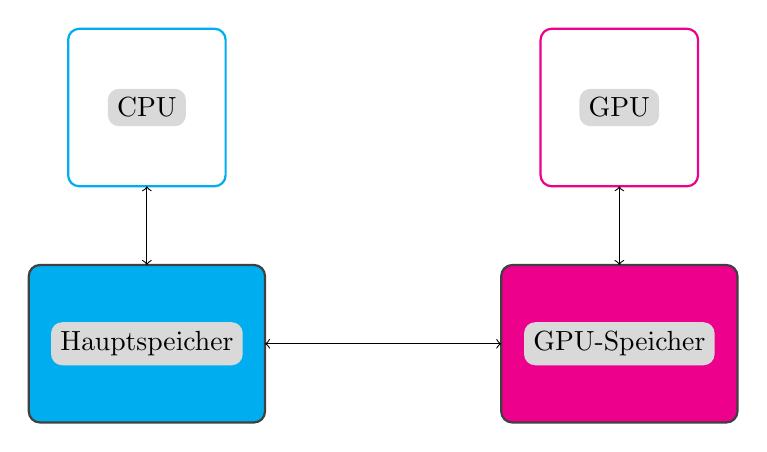
\begin{tikzpicture}
            \draw [thick, rounded corners, draw = cyan]
                  (-1.0, 0.0) rectangle (1.0, 2.0) node[pos = 0.5]
                  {CPU};

            \draw [thick, rounded corners, fill = cyan, draw = darkgray]
                  (-1.5, -3.0) rectangle (1.5, -1.0) node[pos = 0.5]
                  {Hauptspeicher};

            \draw [thick, rounded corners, draw = magenta]
                  (5.0, 0.0) rectangle (7.0, 2.0) node[pos=0.5] {GPU};

            \draw [thick, rounded corners, fill = magenta, draw = darkgray]
                  (4.5, -3.0) rectangle (7.5, -1.0) node[pos = 0.5]
                  {GPU-Speicher};

            \draw [<->] (0.0, 0.0) -- (0.0, -1.0); % CPU <-> RAM
            \draw [<->] (6.0, 0.0) -- (6.0, -1.0); % GPU <-> GPU-RAM
            \draw [<->] (1.5, -2.0) -- (4.5, -2.0); % RAM <-> GPU-RAM
        \end{tikzpicture}
        \caption{Sicht auf den Adressraum bei expliziter Datenbewegung.}
        \label{vergleich:anforderungen:datensicht:explizitebewegung}
    \end{subfigure}
    \par\bigskip
    \begin{subfigure}{0.75\textwidth}
        \centering
        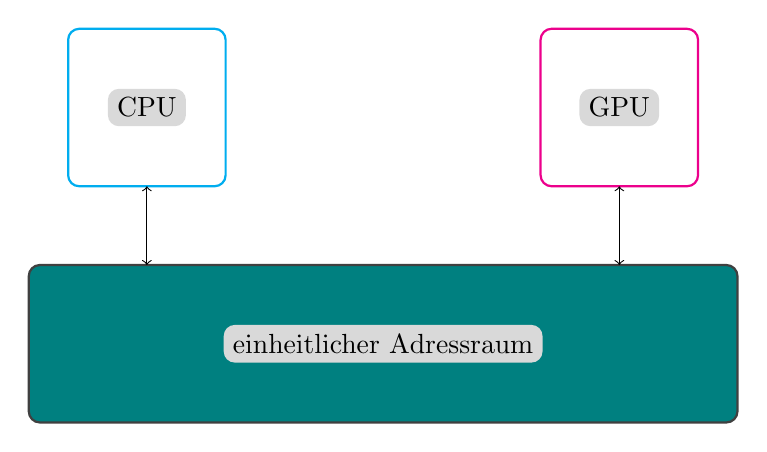
\begin{tikzpicture}
            \draw [thick, rounded corners, draw = cyan]
                  (-1.0, 0.0) rectangle (1.0, 2.0) node[pos = 0.5]
                  {CPU};

            \draw [thick, rounded corners, draw = magenta]
                  (5.0, 0.0) rectangle (7.0, 2.0) node[pos=0.5] {GPU};

            \draw [thick, rounded corners, fill = teal, draw = darkgray]
                  (-1.5, -3.0) rectangle (7.5, -1.0) node[pos = 0.5]
                  {einheitlicher Adressraum};

            \draw [<->] (0.0, 0.0) -- (0.0, -1.0); % CPU <-> Adressraum
            \draw [<->] (6.0, 0.0) -- (6.0, -1.0); % GPU <-> Adressraum
        \end{tikzpicture}
        \caption{Sicht auf den Adressraum bei impliziter Datenbewegung.}
        \label{vergleich:anforderungen:datensicht:implizitebewegung}
    \end{subfigure}
    \caption{Verschiedene Adressraumsichten}
    \label{vergleich:anforderungen:datensicht:adressraeume}
\end{figure}

Eine bewertende Gegenüberstellung beider Ansätze übersteigt den Rahmen dieser
Arbeit (und ist bisher auch in der Literatur nicht zu finden). Stattdessen wird
untersucht, in welcher Form beide Ansätze von den jeweiligen Spracherweiterungen
unterstützt werden.

\paragraph{Datenanordnung}

Die Anordnung der Daten im Speicher kann aufgrund einer Reihe von Faktoren, wie
etwa unterschiedlicher optimaler Zugriffsmuster von CPUs (\textit{cachelines})
und GPUs (\textit{strided access}), erheblich zur Performanz der Berechnung
beitragen. Aus Sicht des Programmieres ist es daher wünschenswert, dass die
Spracherweiterung eine abstrakte Sicht auf den von ihr verwendeten Speicher
bietet, welche die optimalen Zugriffsmuster der verschiedenen Hardware kapselt.

\paragraph{Datenaffinität}

Die Datenaffinität definiert die Zuordnung und Nähe eines Speicherbereichs zu
einer \textit{bestimmten} Ausführungseinheit, die auf diesen Speicherbereich
zugreifen muss. Im Hinblick auf GPUs meint dies die Zuordnung von im
Hauptspeicher liegenden Daten auf eine oder mehrere GPUs.

\paragraph{Datenlokalität}

Die obigen Punkte sind alle eng mit dem Aspekt der Datenlokalität verknüpft.
Im GPU-Kontext ist vornehmlich relevant, inwiefern sich die einzelnen
Ebenen der Speicherhierarchie (GPU-globaler Speicher, lokaler Speicher und Cache
der auf der GPU verbauten parallelen Prozessoren, Register der einzelnen
Threads) durch die Spracherweiterungen ansteuern und nutzen lassen.

\subsubsection{Aufgabensicht}
\label{vergleich:anforderungen:aufgabensicht}

Die im vorherigen Abschnitt genannten Punkte stellen die in dieser Arbeit
verwendeten Vergleichskriterien dar, bedürfen jedoch noch einer Ergänzung:

\paragraph{Aufgabengraphen}

Die Abfolge und Abhängigkeiten einzelner \textit{Kernel} lassen sich in Form
eines Graphen darstellen (siehe
Abbildung~\ref{vergleich:anforderungen:aufgabensicht:graph}). Eine effiziente
Ausnutzung der Parallelität voneinander unabhängiger Aufgaben setzt voraus,
dass Kernel \textit{asynchron} -- sowohl im Hinblick auf die CPU als auch
untereinander -- und \textit{parallel} auf der gleichen GPU ausgeführt werden
können. Im Rahmen dieser Arbeit wird deshalb ebenfalls untersucht, welche Mittel
die einzelnen Spracherweiterungen zur Verfügung stellen, um Aufgabengraphen zu
implementieren.

\begin{figure}[htb]
    \centering
    \begin{tikzpicture}
        \tikzstyle{every node} = [node distance = 3cm, fill = gray!30]

        \Vertex{B}
        \NOEA(B){A}
        \SOEA(B){D}
        \NOEA(D){C}

        \tikzstyle{EdgeStyle}=[post]
        \Edge(A)(B)
        \Edge(A)(C)
        \Edge(B)(D)
        \Edge(C)(D)
    \end{tikzpicture}
    \caption{Beispielhafter Aufgabengraph. Der Kernel D hängt von den Kerneln
             B und C ab, die voneinander unabhängig sind, jedoch beide vom
             Kernel A abhängen.}
    \label{vergleich:anforderungen:aufgabensicht:graph}
\end{figure}

\subsection{CUDA}
\label{vergleich:cuda}

\subsubsection{Übersicht}
\label{vergleich:cuda:uebersicht}

Da der CUDA-Compiler \texttt{nvcc} ein C++-Compiler ist, lässt sich CUDA neben
C++ auch in klassischen C-Programmen nutzen, sofern die Inkompatibilitäten
zwischen C und C++ beachtet werden. Zu diesem Zweck ist das \gls{api} auf
C-Konventionen beschränkt und unterstützt C++-Idiome nur sehr begrenzt. Die
CUDA-Kernel selbst werden in einem C++-Dialekt geschrieben.
(vgl.~\cite{cudaguide}, Abschnitt F)

CUDA-Kernel werden gemeinsam mit dem sie aufrufenden Quelltext kompiliert; CUDA
folgt damit dem Modell der \textit{\gls{singlesource}}\footnote{CUDAs frühester
Konkurrent \gls{opencl} kompiliert die Device-Kernel dagegen erst zur Laufzeit
des Programms, um zwischen verschiedenen Architekturen portabel zu bleiben
(\textit{\gls{splitsource}}.)}. \texttt{nvcc} extrahiert dazu die Kernel und
Device-Funktionen aus dem Quelltext und reicht den verbleibenden C- oder
C++-Quelltext an den auf dem System befindlichen entsprechenden Compiler
weiter. Der Device-Quelltext wird in einem weiteren Schritt vom tatsächlichen
Device-Compiler \texttt{cicc} in die Maschinensprache der Ziel-GPU übersetzt.

\subsubsection{Ausführungsmodell}

Ein \textit{thread} ist die kleinste selbstständige Einheit, die eine Aufgabe
ausführen kann und direkt auf einen Hardware-Thread eines Multiprozessors
abbildbar. \textit{Threads} sind auf der Hardware-Ebene in \textit{warps}
(Gruppen aus 32 Threads) zusammengefasst, die synchron die selben Instruktionen
ausführen. \textit{Warps} entsprechen damit Registern der CPU, die das Modell
\gls{simd} unterstützen, sind im Vergleich zu diesen allerdings flexibler
programmierbar. Dieses Hardware-Modell wird von NVIDIA auch als \gls{simt}
bezeichnet.

Die nächsthöhere Ebene bilden \textit{blocks}, die aus bis zu \num{1024}
\textit{threads} in drei Dimensionen bestehen können (das Produkt der
\textit{thread}-Zahl in $x$-, $y$- und $z$-Richtung darf \num{1024} also nicht
übersteigen). Während die Anzahl der \textit{threads} in diesem Rahmen frei
wählbar ist, bedingt die feste \textit{warp}-Größe, dass eine
\textit{block}-Größe ein Vielfaches von 32 sein sollte, da andernfalls
überzählige \textit{threads} versteckt ausgeführt werden. Ein \textit{block}
wird genau einem Multiprozessor zugeordnet und von diesem ausgeführt. Sind mehr
\textit{blocks} als Multiprozessoren vorhanden, werden \textit{blocks}, die
z.B.\ durch Speicherzugriffe blockiert sind, von ihren Multiprozessoren entfernt
und durch wartende \textit{blocks} ersetzt. Dieser Kontextwechsel geschieht auf
einer GPU deutlich schneller als auf einer CPU und ist nur mit wenigen Zyklen
verbunden.

Alle \textit{threads} eines \textit{blocks} können untereinander über den
Speicher des Multiprozessors kommunizieren (\textit{shared memory}). Barrieren
ermöglichen die Synchronisation zwischen \textit{warps}, während
\textit{threads} innerhalb eines \textit{warps} durch spezielle Intrinsiken
kommunizieren können.

Die Gesamtheit der \textit{blocks} bildet das \textit{grid}, das ebenfalls bis
zu drei Dimensionen umfassen kann. Eine Synchronisierung zwischen
\textit{blocks} ist mit CUDA selbst nicht möglich, allerdings ermöglicht
das im Zusammenhang mit CUDA 9 eingeführte (vgl.~\cite{cuda2018}, S.\ 3)
\gls{api} \textit{cooperative groups} eine \textit{grid}-weite Barriere.
(vgl.~\cite{cudaguide}, Abschnitt 2.2)

\subsubsection{Datensicht}
\label{vergleich:cuda:datensicht}

\paragraph{Datenbewegung}

CUDA bietet mehrere Möglichkeiten der Datenbewegung an. Die \textit{explizite}
Datenbewegung wird seit der ersten CUDA-Version unterstützt und erfordert vom
Programmierer die Allokation von Host- und Device-Speicher, das Auslösen des
Kopiervorgangs der Daten vom Host auf das Device (und zurück) und das Freigeben
des Speichers, wenn er nicht mehr benötigt wird (siehe
Quelltext~\ref{vergleich:cuda:datensicht:explizitebewegung}).

\begin{code}
    \begin{minted}[breaklines,breakafter=\,,escapeinside=||,fontsize=\small]{c++}
auto a_h = new float[num_elems];
auto b_h = new float[num_elems];

/* a_h initialisieren */

auto a_d = static_cast<float*>(nullptr);
auto b_d = static_cast<float*>(nullptr);
cudaMalloc(&a_d, num_elems * sizeof(float));
cudaMalloc(&b_d, num_elems * sizeof(float));

cudaMemcpy(a_d, a_h, num_elems * sizeof(float),
           |\textbf{\textcolor{keyword-green}{cudaMemcpyHostToDevice}}|);

kernel<<<...>>>(a_d, b_d, num_elems);

cudaMemcpy(b_h, b_d, num_elems * sizeof(float),
           |\textbf{\textcolor{keyword-green}{cudaMemcpyDeviceToHost}}|);

cudaFree(b_d);
cudaFree(a_d);

delete[] b_h;
delete[] a_h;
    \end{minted}
    \caption{Explizite Datenbewegung mit CUDA}
    \label{vergleich:cuda:datensicht:explizitebewegung}
\end{code}

Seit dem im Jahr 2011 erschienenen CUDA 4 unterstützt CUDA einen einheitlichen
virtuellen Adressraum für Host und Device (vgl.~\cite{cuda2011}, S.\ 4). Dieser
ermöglichte noch keine implizite Datenbewegung, ersparte dem Programmierer
aber die Angabe der Kopierrichtung beim Aufruf von
\mintinline{c++}{cudaMemcpy}. Der letzte Parameter des Befehls konnte seit
diesem Zeitpunkt durch \mintinline{c++}{cudaMemcpyDefault} ersetzt werden.

Die \textit{implizite} Datenbewegung wird seit dem im Jahr 2014 erschienenen
CUDA 6 unterstützt (vgl.~\cite{cuda2014}, S.\ 3). Der Befehl
\mintinline{c++}{cudaMallocManaged} allokiert einen Speicherbereich, der sowohl
vom Host als auch vom Device angesteuert werden kann. Die CUDA-Laufzeitumgebung
sorgt dann im Hintergrund für das Kopieren der notwendigen Speicherbereiche. Es
obliegt jedoch dem Programmierer, die Synchronisierung zwischen Host und Device
auszuführen. Das in Quelltext~\ref{vergleich:cuda:datensicht:explizitebewegung}
aufgeführte Beispiel wird dadurch zu der in
Quelltext~\ref{vergleich:cuda:datensicht:implizitebewegung} gezeigten
Vereinfachung.

\begin{code}
    \begin{minted}[breaklines,breakafter=\,,escapeinside=||,fontsize=\small]{c++}
auto a = static_cast<float*>(nullptr);
auto b = static_cast<float*>(nullptr);

cudaMallocManaged(&a, num_elems * sizeof(float));
cudaMallocManaged(&b, num_elems * sizeof(float));

kernel<<<...>>>(a, b, num_elems);

cudaDeviceSynchronize();

/* b ab hier auf dem Host nutzbar */

cudaFree(b);
cudaFree(a);
    \end{minted}
    \caption{Implizite Datenbewegung ab CUDA 6}
    \label{vergleich:cuda:datensicht:implizitebewegung}
\end{code}

Im Jahr 2016 führte NVIDIA die Pascal-Architektur und CUDA 8 ein. Mit dieser
neuen Architektur wurde die implizite Datenbewegung weiter vereinfacht, da es
nun möglich war, gänzlich auf CUDA zur Speicherallokation zu verzichten: der
Aufruf von \mintinline{c++}{new} oder \mintinline{c}{malloc} genügt
(vgl.~\cite{harris2016}). Dadurch wurde auch die Verwendung von C++-Containern
im Zusammenhang mit CUDA einfacher, deren Speicherbereich man nun direkt an
CUDA-Kernel übergeben konnte (siehe
Quelltext~\ref{vergleich:cuda:datensicht:explizitcuda8}).

\begin{code}
    \begin{minted}[breaklines,breakafter=\,,escapeinside=||,fontsize=\small]{c++}
auto a = std::vector<float>{};
auto b = std::vector<float>{};

a.resize(num_elems);
b.resize(num_elems);

kernel<<<...>>>(a.data(), b.data(), num_elems);

cudaDeviceSynchronize();

/* b ab hier auf dem Host nutzbar */
    \end{minted}
    \caption{Implizite Datenbewegung ab CUDA 8 und Pascal}
    \label{vergleich:cuda:datensicht:explizitcuda8}
\end{code}

\paragraph{Datenanordnung}

Die Anordnung der Daten im globalen Speicher der GPU entspricht bei der
Allokation mit \mintinline{c++}{cudaMalloc} und der Kopie mit
\mintinline{c++}{cudaMemcpy} der Anordnung der Daten im Host-Speicher. Es ist
Aufgabe des Programmierers, die Effizienz der Anordnung und des
Zugriffsverhaltens sicherzustellen (vgl.~\cite{cudaguide}, Abschnitt 5.3.2,
Überschrift \glqq Global Memory\grqq).

Einen Sonderfall stellen zweidimensionale Arrays dar. Die Adresse $A$ eines
Felds eines 2D-Arrays mit der Startadresse $S$ und der Breite $B$ durch einen
Thread mit den Koordinaten $(x, y)$ berechnet sich in vielen Anwendungsfällen
wie folgt:

\begin{align*}
    A = S + y * B + x
\end{align*}

Ein effizienter Zugriff dieser Form erfordert sowohl eine Block-Breite als auch
eine Array-Breite, die ein mathematisches Vielfaches der Warpbreite sind. Mit
\mintinline{c++}{cudaMallocPitch} und \mintinline{c++}{cudaMemcpy2D} kann man
letzterer Anforderung Rechnung tragen. Eine Erweiterung dieses Prinzips auf
dreidimensionale Arrays, die man sich auch als Array von 2D-Arrays vorstellen
kann, ist mit \mintinline{c++}{cudaMalloc3D} und \mintinline{c++}{cudaMemcpy3D}
möglich. (vgl.~\cite{cudaguide}, Abschnitt 5.3.2, Überschrift \glqq
Two-Dimensional Arrays\grqq)

Sofern häufig auf benachbarte Spalten und Zeilen eines Arrays zugegriffen
wird, lässt sich dies effizienter auslesen, wenn die eigentlich für
Grafikoperationen -- die häufig benachbarte Pixel manipulieren -- vorgesehenen
Textur-Caches der GPU genutzt werden. Eine für diese Caches optimale
Speicheranordnung lässt sich mit \mintinline{c++}{cudaMallocArray}
bewerkstelligen. Ein auf diese Weise angelegtes \mintinline{c++}{cudaArray} ist
kein Zeiger, sondern eine für den Programmierer opake Datenstruktur, auf die
nur über spezielle Texturbefehle zugegriffen werden kann.
(vgl.~\cite{cudaguide}, Abschnitt 5.3.2, Überschrift \glqq Texture and Surface
Memory\grqq)

\paragraph{Datenaffinität}

Die explizite Datenbewegung ordnet die kopierten Daten automatisch der
\textit{aktiven} GPU zu. Der CUDA-Kontext kennt generell nur ein aktives Device;
will man in einem Multi-GPU-System auf eine andere GPU wechseln, geschieht dies
durch den manuellen Wechsel mit dem Befehl \texttt{cudaSetDevice} (siehe
Quelltext~\ref{vergleich:cuda:datensicht:setdevice}).

Dieses Verfahren gilt zum Teil auch für die implizite Datenbewegung. Speicher,
der mit dem Befehl \texttt{cudaMallocManaged} reserviert wurde, wird bei allen
NVIDIA-GPU-Architekturen bis einschließlich \textit{Maxwell} nur zwischen dem
Host und dem zum Zeitpunkt der Reservierung aktiven Device ausgetauscht. Ab der
\textit{Kepler}-Architektur wird der Speicher dagegen auf allen GPUs sichtbar
und nach Bedarf auf die GPU kopiert, welche die Daten benötigt.
(vgl.~\cite{cudaguide}, Abschnitt K.1.5)

\begin{code}
    \begin{minted}[fontsize=\small]{c++}
auto count = 0;
cudaGetDeviceCount(&count); // Zahl der GPUs abfragen

cudaSetDevice(0); // Device 0 aktiv
cudaMemcpy(..., cudaMemcpyHostToDevice); // kopieren auf Device 0

cudaSetDevice(1); // Device 1 aktiv
cudaMemcpy(..., cudaMemcpyHostToDevice); // kopieren auf Device 1
    \end{minted}
    \caption{Setzen der aktiven GPU mit CUDA}
    \label{vergleich:cuda:datensicht:setdevice}
\end{code}

\paragraph{Datenlokalität}

CUDA kennt sieben Ebenen innerhalb der GPU-Speicherhierarchie
(vgl.~\cite{cudaguide}, Abschnitt 5.3.2).

\textit{Global memory} ist der Hauptspeicher der GPU und für alle
Multiprozessoren sichtbar. Die Zugriffe sind jedoch zeitaufwendig.

Zugriffe auf den \textit{global memory} erfolgen über L1- (pro Multiprozessor)
und L2-Caches (alle Multiprozessoren). Die Caches lassen sich vom Programmierer
nicht direkt ansteuern.

\textit{Constant memory} ist ein spezieller Cache, der vom Programmierer selbst
befüllt werden muss. Er ermöglicht deutlich schnellere Speicherzugriffe, wenn
alle \textit{threads} eines \textit{warps} gleichzeitig auf das gleiche Datum
zugreifen.

Operationen, die die Textureinheiten der GPU verwenden, können über die
Textur-Caches der GPU lesend auf den \textit{global memory} zugreifen. Diese
Caches sind für häufige zweidimensionale Speicherzugriffe auf benachbarte Zeilen
und Spalten optimiert. Sie sind vom Programmierer mittels der Intrinsik
\texttt{\_\_ldg} direkt ansprechbar oder können implizit durch die in CUDA
enthaltenen Texturbefehle genutzt werden.

\textit{Shared memory} ist ein spezieller L1-Cache, der direkt vom Programmierer
lesbar und beschreibbar ist. Der \textit{shared memory} ist in seiner Kapazität
sehr eingeschränkt (er umfasst nur einige KiB), ermöglicht dem Programmierer
aber sehr schnelle Zugriffe sowie die Kommunikation zwischen \textit{threads}
eines \textit{blocks}.

Die Register des Multiprozessors werden \textit{threads} nach Bedarf zugeordnet
und sind vom Programmierer nicht direkt ansprechbar.

\textit{Local memory} ist \textit{thread}-lokaler \textit{global memory}. In
diesem werden lokale Variablen, die nicht mehr in die Register passen
(weil deren Anzahl erschöpft ist), oder Arrays unbekannter Länge automatisch
untergebracht. Da der \textit{local memory} versteckt im \textit{global memory}
liegt, ist seine Nutzung aufgrund der langen Zugriffszeiten üblicherweise
unerwünscht.

\subsubsection{Aufgabensicht}

\paragraph{Aufgabengraphen}

Aufgabengraphen lassen sich in CUDA auf zwei Arten implementieren. Der
herkömmliche Weg ist die Verwendung von \textit{streams}. Diese können als
Warteschlangen für Aufgaben (Speicherbewegungen, Kernel-Ausführungen) gesehen
werden und sind untereinander und in Bezug auf den Host asynchron. Das heißt,
dass verschiedene Kernel in getrennten \textit{streams} parallel auf der GPU
ausgeführt werden können (entsprechende Hardware-Ressourcen vorausgesetzt).
Innerhalb eines \textit{streams} sind alle Aufgaben immer serialisiert, zwei
Kernel im selben \textit{stream} werden also immer nacheinander ausgeführt.

Die Kommunikation bzw.\ Synchronisation zwischen \textit{streams} erfolgt über
\textit{events}. \textit{Events} werden z.B.\ durch das Beenden eines Kernels
ausgelöst. Ist ein Kernel eines anderen \textit{streams} von diesem abhängig,
lässt sich durch das Warten auf dieses \textit{event} der \textit{stream}
blockieren, bis die Ausführung fortgesetzt werden kann.

Der Quelltext~\ref{vergleich:cuda:aufgabensicht:streams} zeigt die
Implementierung des Beispiel-Graphen
in Abbildung~\ref{vergleich:anforderungen:aufgabensicht:graph} mit
\textit{streams}.

\begin{code}
    \begin{minted}[fontsize=\small]{c++}
        A<<<..., stream1>>>();
        // eventA wird ausgelöst, sobald A fertig ist
        cudaEventRecord(eventA, stream1);

        B<<<..., stream1>>>(); // wartet automatisch auf A

        // stream2 wartet auf eventA
        cudaStreamWaitEvent(stream2, eventA);
        // C kann jetzt ausgeführt werden
        C<<<..., stream2>>>();
        // eventC wird ausgelöst, sobald C fertig ist
        cudaEventRecord(eventC, stream2);

        // stream1 wartet auf eventC
        cudaStreamEvent(stream1, eventC);
        D<<<..., stream1>>>(); // wartet automatisch auf B
    \end{minted}
    \caption{Aufgabengraph mit \textit{streams}}
    \label{vergleich:cuda:aufgabensicht:streams}
\end{code}

Der \textit{stream}-Ansatz hat den Nachteil, dass bei iterativen Verfahren, die
das mehrfache Ausführen des Graphen erfordern, durch das ständige Starten der
Kernel und das manuelle Blockieren der \textit{streams} viel Overhead erzeugt
wird. Die mit dem 2018 veröffentlichten CUDA 10 eingeführten
\textit{CUDA Graphs} (vgl.~\cite{cuda10rel}, S.\ 4) sollen dieses Problem lösen
(vgl.~\cite{ramarao2018} für eine Einführung).

Aufgabengraphen lassen sich mit diesem \gls{api} direkt implementieren.
Quelltext~\ref{vergleich:cuda:aufgabensicht:graph} zeigt die
Abbildung~\ref{vergleich:anforderungen:aufgabensicht:graph} entsprechende
Implementierung. 

\begin{code}
    \begin{minted}[fontsize=\small]{c++}
        cudaGraphCreate(&graph);

        // Abhängigkeiten definieren
        cudaGraphAddNode(graph, A, {}, ...);
        cudaGraphAddNode(graph, B, {A}, ...);
        cudaGraphAddNode(graph, C, {A}, ...);
        cudaGraphAddNode(graph, D, {B, C}, ...);

        // Graph-Instanz erzeugen
        cudaGraphInstantiate(&instance, graph);

        // Graph-Instanz auf stream ausführen
        cudaGraphLaunch(instance, stream);
    \end{minted}
    \caption{Aufgabengraph mit \textit{CUDA Graphs}}
    \label{vergleich:cuda:aufgabensicht:graph}
\end{code}

\subsection{HIP}

\subsubsection{Übersicht}

AMDs \gls{hip}-\gls{api} ist als portable Alternative zu CUDA gedacht und de
facto ein Klon des CUDA-\gls{api}, bei dem fast jeder CUDA-Befehl
\texttt{cudaCmd} seine genaue Entsprechung im \gls{hip}-Befehl \texttt{hipCmd}
findet. Tatsächlich werden \gls{hip}-Quelltexte, die für eine NVIDIA-GPU
kompiliert werden sollen, von einem einfachen Skript wieder in CUDA-Quelltexte
umgewandelt. Diese werden dann vom \texttt{nvcc}-Compiler übersetzt.

Die in den vorherigen Abschnitten für CUDA dargestellten Prinzipien gelten daher
weitestgehend auch für \gls{hip}; vorhandene Unterschiede werden in den
folgenden Abschnitten aufgeführt.

\gls{hip} für AMD-GPUs ist eine dünne Schicht über AMDs eigentlichem
\gls{gpgpu}-\gls{api}, \gls{hc}, das in Abschnitt~\ref{vergleich:hc} vorgestellt
wird.

\subsubsection{Datensicht}

\paragraph{Datenbewegung}

Die implizite Datenbewegung, die mit \texttt{cudaMallocManaged} möglich ist,
hat gegenwärtig kein \gls{hip}-Äquivalent. Programmierer haben daher nur die
Möglichkeit der expliziten Datenbewegung.

\paragraph{Datenanordnung}

Zweidimensionaler Speicher kann auf CUDA-GPUs mit \texttt{cudaMallocPitch} in
einer optimierten Anordnung reserviert werden. Dieser Befehl wird derzeit nicht
in \gls{hip} abgebildet. Gleiches gilt für \texttt{cudaArray}s, die in ihrer
Anordnung für den Textur-Cache optimiert sind.

\paragraph{Datenlokalität}

Die Textur-Einheiten und damit der Textur-Cache der GPU werden von \gls{hip} zur
Zeit nur eingeschränkt unterstützt.

\subsubsection{Aufgabensicht}

\paragraph{Aufgabengraphen}

Aufgabengraphen lassen sich in \gls{hip} nur über \textit{streams}
implementieren, \textit{CUDA Graphs} werden momentan nicht unterstützt.

\subsection{HC}
\label{vergleich:hc}

\subsubsection{Übersicht}

\subsubsection{Ausführungsmodell}

\subsubsection{Datensicht}

\paragraph{Datenbewegung}

\paragraph{Datenanordnung}

\paragraph{Datenaffinität}

\paragraph{Datenlokalität}

\subsubsection{Aufgabensicht}

\paragraph{Aufgabengraphen}

\subsection{SYCL}
\label{vergleich:sycl}

\subsubsection{Übersicht}

\subsubsection{Ausführungsmodell}

\subsubsection{Datensicht}

\paragraph{Datenbewegung}

\paragraph{Datenanordnung}

\paragraph{Datenaffinität}

\paragraph{Datenlokalität}

\subsubsection{Aufgabensicht}

\paragraph{Aufgabengraphen}

\subsection{Zusammenfassung}
\label{vergleich:zusammenfassung}
